
\chapter{Boundary Value Problems}

So far, we have focused exclusively on IVPs, where the state of the system and its derivatives are fully known at a single starting point, $t_0$. The solver's task was simply to march forward in time. However, many physical problems, particularly those involving space rather than time, provide information at two different boundaries. These are known as \textbf{boundary value problems (BVPs)}. Formally, a BVP consists of a system of differential equations defined on an interval $[t_0, t_f]$:
\begin{equation}
    \frac{d\mathbf{x}}{dt} = \mathbf{f}(\mathbf{x}, t)
\end{equation}
coupled with a set of boundary conditions (BCs) that relate the state at the start and the end of the interval:
\begin{equation}
    \mathbf{g}(\mathbf{x}(t_0), \mathbf{x}(t_f)) = 0
\end{equation}
Here, $\mathbf{x}: [t_0, t_f] \to \mathbb{R}^N$ is the state vector, and the independent variable $t$ often represents space (e.g., position along a beam) rather than time. Unlike IVPs, where existence and uniqueness are usually guaranteed by Lipschitz continuity, BVPs are much harder to solve and may have no solution, a unique solution, or infinitely many solutions depending on the boundary conditions.

\begin{exampleBox}
    \textbf{Example: Reaction-Diffusion in a Slab}
    
    Consider the steady-state concentration $C(x)$ of a chemical species diffusing through a slab while undergoing a reaction $r(C)$. The governing equation is a second-order ODE:
    \begin{equation}
        \frac{d^2C}{dx^2} = -r(C)
    \end{equation}
    To solve this, we must convert it to a system of first-order ODEs. Let $\mathbf{y} = [C, C']^\top$. The system becomes:
    \begin{equation}
        \frac{d}{dx} \begin{bmatrix} C \\ C' \end{bmatrix} = \begin{bmatrix} C' \\ -r(C) \end{bmatrix}
    \end{equation}
    Usually, we know the concentration at the surface ($x=0$) and perhaps that the flux is zero at the center ($x=1$). These form the boundary conditions:
    \begin{equation}
        C(0) = 1, \quad C'(1) = 0 \quad \implies \quad \mathbf{g}(\mathbf{y}(0), \mathbf{y}(1)) = \begin{bmatrix} C(0) - 1 \\ C'(1) \end{bmatrix} = \mathbf{0}
    \end{equation}
\end{exampleBox}

\section{Introduction to Boundary Value Problems}

\subsection{Classification of Boundary Conditions}

The function $\mathbf{g}$ can take many forms, but in engineering, three specific types of boundary conditions appear most frequently.

\textbf{Dirichlet boundary conditions} specify the value of the solution itself at the boundaries. For a second-order system, this might look like $C(0) = 1$ and $C(1) = 0$. In vector notation, this restricts specific components of the state vector $\mathbf{x}$; i.e., $\mathbf{B}_0 \mathbf{x}(t_0) + \mathbf{B}_1 \mathbf{x}(t_f) = \mathbf{b}$.

\textbf{Neumann boundary conditions} specify the value of the derivative (flux) at the boundaries. For example, $C'(0) = 1$ and $C'(1) = 0$. In the first-order system formulation, this corresponds to constraining the specific vector components that represent velocities or fluxes.

\textbf{Robin boundary conditions} are linear combinations of Dirichlet and Neumann conditions. These often arise in convection problems (Newton's law of cooling) or elastic supports. Mathematically, they take the form:
\begin{equation}
    a_1 C(0) + a_2 C'(0) = 1 \quad \text{and} \quad b_1 C(1) + b_2 C'(1) = 0
\end{equation}
In the first-order system formulation, all of these conditions (Dirichlet, Neumann, and Robin) are simply algebraic constraints on the state vector at the boundaries, generalized as $\mathbf{B}_0 \mathbf{x}(t_0) + \mathbf{B}_1 \mathbf{x}(t_f) = \mathbf{b}$.

\subsection{Linear BVPs}

Before tackling the general nonlinear case, we consider linear BVPs, where both the differential equations and the boundary conditions are linear. The problem is formulated as
\begin{equation}
    \frac{d\mathbf{x}}{dt} = \mathbf{A}\mathbf{x}, \quad \mathbf{B}_0 \mathbf{x}(0) + \mathbf{B}_T \mathbf{x}(T) + \mathbf{b} = 0
\end{equation}
where $\mathbf{A}$ is a constant matrix. If we assume $\mathbf{A}$ is diagonalizable with eigenvectors $\mathbf{W}$ and eigenvalues $\mathbf{\Lambda}$, we already know the general solution to the ODE from our study of IVPs. If we impose an arbitrary initial condition $\mathbf{x}(0) = \mathbf{c}$, the solution at time $t$ is:
\begin{equation}
    \mathbf{x}(t) = \mathbf{W} e^{\mathbf{\Lambda} t} \mathbf{W}^{-1} \mathbf{c}
\end{equation}
The unique challenge of the BVP is that we do not know $\mathbf{c}$; it is an unknown vector we must find. However, we can substitute the analytical solution form into the boundary condition equation:
\begin{equation}
    \mathbf{B}_0 \mathbf{c} + \mathbf{B}_T \left( \mathbf{W} e^{\mathbf{\Lambda} T} \mathbf{W}^{-1} \mathbf{c} \right) + \mathbf{b} = 0
\end{equation}
Factoring out the unknown vector $\mathbf{c}$, we arrive at a system of linear algebraic equations:
\begin{equation}
    \left( \mathbf{B}_0 + \mathbf{B}_T \mathbf{W} e^{\mathbf{\Lambda} T} \mathbf{W}^{-1} \right) \mathbf{c} = -\mathbf{b}
\end{equation}
This result is powerful because it reduces a calculus problem to a linear algebra problem $\mathbf{M}\mathbf{c} = -\mathbf{b}$. A solution exists if the vector $\mathbf{b}$ lies in the column space (range) of the matrix $\mathbf{M} = \mathbf{B}_0 + \mathbf{B}_T \mathbf{W} e^{\mathbf{\Lambda} T} \mathbf{W}^{-1}$. Furthermore, a \textit{unique} solution exists if and only if the determinant of this matrix is non-zero:
\begin{equation}
    \det \left( \mathbf{B}_0 + \mathbf{B}_T \mathbf{W} e^{\mathbf{\Lambda} T} \mathbf{W}^{-1} \right) \neq 0
\end{equation}
If a unique solution exists, we can solve for $\mathbf{c}$ simply by inverting the matrix:
\begin{equation}
    \mathbf{c} = - \left( \mathbf{B}_0 + \mathbf{B}_T \mathbf{W} e^{\mathbf{\Lambda} T} \mathbf{W}^{-1} \right)^{-1} \mathbf{b}
\end{equation}
Once $\mathbf{c}$ is found, the full solution $\mathbf{x}(t)$ is obtained by propagating this initial condition forward. In particular, combining this with the general solution $\mathbf{x}(t) = \mathbf{W}e^{\mathbf{\Lambda} t}\mathbf{W}^{-1}\mathbf{c}$, we can write the full solution explicitly as
\begin{align}
    \mathbf{x}(t)
    &= \mathbf{W} e^{\mathbf{\Lambda} t} \mathbf{W}^{-1} \mathbf{c} \nonumber \\
    &= -\,\mathbf{W} e^{\mathbf{\Lambda} t} \mathbf{W}^{-1}
       \left( \mathbf{B}_0 + \mathbf{B}_T \mathbf{W} e^{\mathbf{\Lambda} T} \mathbf{W}^{-1} \right)^{-1}
       \mathbf{b}
\end{align}


\begin{exampleBox}
    \textbf{Example: }
    Consider the boundary value problem
    \begin{equation}
        \frac{d\mathbf{x}}{dt} = \mathbf{A}\mathbf{x},\qquad
        \mathbf{A} = \begin{bmatrix}1 & 0\\[4pt] 0 & -1\end{bmatrix},\qquad
        \mathbf{x}(t) \in \mathbb{R}^2
    \end{equation}
    with final time $T=1$ and boundary conditions
    \begin{equation}
        x_1(0) = 0,\qquad x_2(1) = 1
    \end{equation}
    We write these boundary conditions in the form
    \begin{equation}
        \mathbf{B}_0 \mathbf{x}(0) + \mathbf{B}_T \mathbf{x}(1) + \mathbf{b} = 0
    \end{equation}
    with
    \begin{equation}
        \mathbf{B}_0 = \begin{bmatrix}1 & 0\\[4pt] 0 & 0\end{bmatrix},\quad
        \mathbf{B}_T = \begin{bmatrix}0 & 0\\[4pt] 0 & 1\end{bmatrix},\quad
        \mathbf{b} = \begin{bmatrix}0\\[4pt] -1\end{bmatrix}
    \end{equation}
    since this gives
    \begin{equation}
        \mathbf{B}_0\mathbf{x}(0) + \mathbf{B}_T\mathbf{x}(1) + \mathbf{b}
        =
        \begin{bmatrix}x_1(0)\\[4pt] x_2(1) - 1\end{bmatrix}
        = \mathbf{0}
    \end{equation}

    The matrix $A$ is already diagonal:
    \begin{equation}
        \mathbf{A} = \mathbf{W}\mathbf{\Lambda} \mathbf{W}^{-1},\qquad
        \mathbf{W} = \mathbf{I},\quad
        \mathbf{\Lambda} = \begin{bmatrix}1 & 0\\[4pt] 0 & -1\end{bmatrix}
    \end{equation}
    For an arbitrary initial condition $\mathbf{x}(0) = \mathbf{c}$, the solution is
    \begin{equation}
        \mathbf{x}(t) = \mathbf{W} e^{\mathbf{\Lambda} t} \mathbf{W}^{-1} \mathbf{c}
        = \begin{bmatrix}e^{t} & 0\\[4pt] 0 & e^{-t}\end{bmatrix} \mathbf{c}
    \end{equation}

    To enforce the boundary conditions, form
    \begin{equation}
        \mathbf{M} \mathbf{c} = -\mathbf{b},\qquad
        \mathbf{M} := \mathbf{B}_0 + \mathbf{B}_T \mathbf{W} e^{\mathbf{\Lambda} T} \mathbf{W}^{-1}
    \end{equation}
    Here $T=1$ and
    \begin{equation}
        e^{\mathbf{\Lambda} T} = e^{\mathbf{\Lambda}} = 
    \begin{bmatrix}e & 0\\[4pt] 0 & e^{-1}\end{bmatrix}
    \end{equation}
    so
    \begin{equation}
        \mathbf{M} = \mathbf{B}_0 + \mathbf{B}_T \mathbf{W} e^{\mathbf{\Lambda} T} \mathbf{W}^{-1}
        = \begin{bmatrix}1 & 0\\[4pt] 0 & 0\end{bmatrix}
        + \begin{bmatrix}0 & 0\\[4pt] 0 & 1\end{bmatrix}
        \begin{bmatrix}e & 0\\[4pt] 0 & e^{-1}\end{bmatrix}
        = \begin{bmatrix}1 & 0\\[4pt] 0 & e^{-1}\end{bmatrix}
    \end{equation}
    Since $\det(\mathbf{M}) = e^{-1} \neq 0$, there is a unique solution:
    \begin{equation}
        \mathbf{M}\mathbf{c} = -\mathbf{b}
        \quad\implies\quad
        \begin{bmatrix}1 & 0\\[4pt] 0 & e^{-1}\end{bmatrix}
        \begin{bmatrix}c_1\\[4pt] c_2\end{bmatrix}
        =
        \begin{bmatrix}0\\[4pt] 1\end{bmatrix}
        \quad\implies\quad
        c_1 = 0,\quad c_2 = e
    \end{equation}
    Thus
    \begin{equation}
        \mathbf{c} = \mathbf{x}(0) =
        \begin{bmatrix}0\\[4pt] e\end{bmatrix}
    \end{equation}
    and the full solution is
    \begin{equation}
        \mathbf{x}(t) = 
        \begin{bmatrix}e^{t} & 0\\[4pt] 0 & e^{-t}\end{bmatrix}
        \begin{bmatrix}0\\[4pt] e\end{bmatrix}
        =
        \begin{bmatrix}0\\[4pt] e^{1-t}\end{bmatrix}
    \end{equation}
    We can easily check that $x_1(0) = 0$ and $x_2(1) = 1$, so the BVP is solved.

\end{exampleBox}

\section{Shooting Methods}

\subsection{The Shooting Method}

When the differential equation $\dot{\mathbf{x}} = \mathbf{f}(\mathbf{x}, t)$ or the boundary conditions are nonlinear, we cannot use linear superposition or matrix inversion. Instead, we employ an iterative numerical approach known as the shooting method. The intuition comes from artillery. Suppose we have a cannon at position $x_0$ and we want to hit a target at $x_T$ at time $T$. We know the starting position, but we do not know the necessary initial velocity (angle and speed). We guess an initial velocity $\mathbf{v}(0)$, fire the cannon (integrate the ODE), and see where the shell lands. Based on the ``miss distance'' (the residual), we adjust the initial velocity (in an intelligent way, using Newton-Raphson) and fire again (\autoref{fig:shooting_diagram}).

Mathematically, this corresponds to us transforming the BVP into a root-finding problem. We temporarily assume we know the full initial state $\mathbf{c} \in \mathbb{R}^N$ such that $\mathbf{x}(0) = \mathbf{c}$. This converts the BVP into an IVP, which we denote as $\mathbf{x}(t; \mathbf{c})$. We can solve this IVP numerically to find the state at the final time, $\mathbf{x}(T; \mathbf{c})$. We then define a residual function $\mathbf{h}$ (where $\mathbf{h}: \mathbb{R}^N \to \mathbb{R}^N$) representing the error in the boundary conditions:
\begin{equation}
    \mathbf{h}(\mathbf{c}) := \mathbf{g}(\mathbf{c}, \mathbf{x}(T; \mathbf{c})) = 0
\end{equation}
Here, $\mathbf{g} : \mathbb{R}^N \times \mathbb{R}^N \to \mathbb{R}^N$ encodes the boundary conditions at both ends. Our goal is to find the root vector $\mathbf{c}^*$ such that $\mathbf{h}(\mathbf{c}^*) = 0$. Since $\mathbf{h}$ is a nonlinear function, we use the Newton-Raphson method.

\paragraph*{Newton-Raphson for Shooting}

To apply Newton-Raphson, we start with an initial guess $\mathbf{c}_i$ and iteratively update it using the Jacobian matrix $\mathbf{J}_{\mathbf{h}}(\mathbf{c}) \in \mathbb{R}^{N \times N}$:
\begin{equation}
    \mathbf{c}_{i+1} = \mathbf{c}_i - (\mathbf{J}_{\mathbf{h}}(\mathbf{c}_i))^{-1} \mathbf{h}(\mathbf{c}_i)
\end{equation}
(Note: In practice, we do not invert the matrix. Instead, we solve the linear system $\mathbf{J}_{\mathbf{h}}(\mathbf{c}_i) \delta \mathbf{c} = -\mathbf{h}(\mathbf{c}_i)$ for the correction $\delta \mathbf{c}$). By the chain rule, this Jacobian depends on how the boundary function $\mathbf{g}$ changes with respect to the initial condition $\mathbf{c}$:
\begin{equation}
    \mathbf{J}_{\mathbf{h}}(\mathbf{c}) = \frac{\partial \mathbf{g}}{\partial \mathbf{c}} + \frac{\partial \mathbf{g}}{\partial \mathbf{x}(T)} \frac{\partial \mathbf{x}(T; \mathbf{c})}{\partial \mathbf{c}}
\end{equation}
The terms $\frac{\partial \mathbf{g}}{\partial \mathbf{c}}$ and $\frac{\partial \mathbf{g}}{\partial \mathbf{x}}$ are algebraic derivatives of the boundary condition function, which are usually easy to calculate. However, the term $\frac{\partial \mathbf{x}(T; \mathbf{c})}{\partial \mathbf{c}}$ corresponds to the sensitivity of the ODE solution at time $T$ to changes in the initial condition at time $0$. This term cannot be found algebraically; it requires solving differential equations.

\subsection{Sensitivity Analysis}

We define the \textbf{sensitivity matrix} $\mathbf{S}(t; \mathbf{c})$ as the derivative of the state with respect to the initial condition:
\begin{equation}
    \mathbf{S}(t; \mathbf{c}) = \frac{\partial \mathbf{x}(t; \mathbf{c})}{\partial \mathbf{c}}
\end{equation}
Here $\mathbf{S}(t; \mathbf{c})$ is an $N \times N$ matrix. In code, we typically flatten it into a vector of length $N^2$ and integrate it alongside $\mathbf{x}$. (Alternatively, we could approximate $\mathbf{J}_{\mathbf{h}}$ via finite differences in $\mathbf{c}$, but integrating the variational equation is usually more accurate and efficient locally).
At time $t=0$, the sensitivity is simply the identity matrix, $\mathbf{S}(0) = \mathbf{I}$, because $\mathbf{x}(0) = \mathbf{c}$. To find how $\mathbf{S}$ evolves over time, we differentiate the original ODE $\frac{d\mathbf{x}}{dt} = \mathbf{f}(\mathbf{x}, t)$ with respect to $\mathbf{c}$. Using the chain rule and switching the order of differentiation:
\begin{equation}
    \frac{d}{dt} \left( \frac{\partial \mathbf{x}}{\partial \mathbf{c}} \right) = \frac{\partial}{\partial \mathbf{c}} \mathbf{f}(\mathbf{x}(t; \mathbf{c}), t) = \frac{\partial \mathbf{f}}{\partial \mathbf{x}} \frac{\partial \mathbf{x}}{\partial \mathbf{c}}
\end{equation}
Substituting $\mathbf{S}$ and the Jacobian of the dynamics $\mathbf{J}(\mathbf{x}, t) = \frac{\partial \mathbf{f}}{\partial \mathbf{x}}$, we arrive at the variational equation, which is a matrix-valued IVP:
\begin{equation}
    \frac{d\mathbf{S}}{dt} = \mathbf{J}(\mathbf{x}, t) \mathbf{S}, \quad \mathbf{S}(0) = \mathbf{I}
\end{equation}
In practice, to perform one iteration of the Newton-Raphson shooting method, we must numerically integrate a coupled system of size $N + N^2$:
\begin{equation}
    \begin{cases}
        \frac{d\mathbf{x}}{dt} = \mathbf{f}(\mathbf{x}, t), & \mathbf{x}(0) = \mathbf{c} \\
        \frac{d\mathbf{S}}{dt} = \mathbf{J}(\mathbf{x}, t)\mathbf{S}, & \mathbf{S}(0) = \mathbf{I}
    \end{cases}
\end{equation}
Solving this coupled system from $t=0$ to $t=T$ yields both the residual $\mathbf{h}(\mathbf{c})$ (via $\mathbf{x}(T)$) and the Jacobian $\mathbf{J}_{\mathbf{h}}(\mathbf{c})$ (via $\mathbf{S}(T)$), allowing us to compute the Newton step.

\begin{figure}[H]
    \centering
    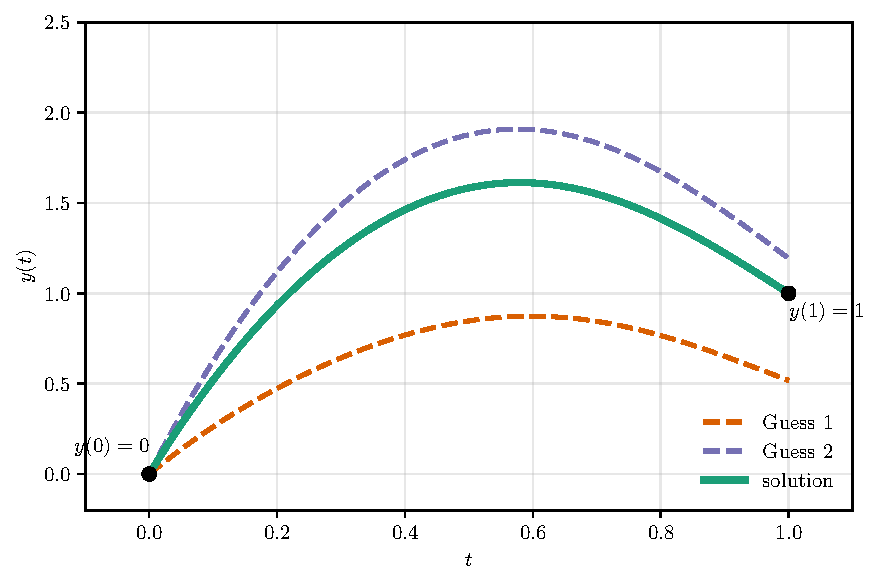
\includegraphics[width=0.7\textwidth]{figs/ode/shooting.pdf}
    \caption{Shooting method for the boundary value problem $y''+2y'+5y = 2\sin(2\pi t)$ with $y(0)=0$ and $y(1)=1$. Two initial guesses for the unknown initial slope produce trajectories that miss the boundary condition at $t=1$, while the final trajectory corresponds to the solution obtained by adjusting the initial slope with a root-finding method.}

    \label{fig:shooting_diagram}
\end{figure}

\subsection{The Multiple Shooting Method}

While the shooting method is conceptually simple, it suffers from a major weakness: sensitivity to initial conditions. The Newton-Raphson update relies on the inverse of the Jacobian $\mathbf{J}_{\mathbf{h}}(\mathbf{c})$. This matrix essentially contains the sensitivity term $\mathbf{S}(T; \mathbf{c})$. If the physical system is chaotic (e.g., the Lorenz system) or simply has rapidly growing modes, the sensitivity $\mathbf{S}(T)$ can become exponentially large. This leads to an ill-conditioned Jacobian. Numerically, this means that a microscopic change in the initial guess $\mathbf{c}$ leads to a massive change in the trajectory $\mathbf{x}(T)$, causing the numerical integrator to diverge or the Newton iterations to overshoot wildly.

\begin{exampleBox}
    \textbf{Sensitivity in the Lorenz System}
    Consider a chaotic Lorenz system:
    \begin{equation}
        \dot{x} = 10(y-x), \quad \dot{y} = x(30-z)-y, \quad \dot{z} = xy - 2z
    \end{equation}
    If we attempt to solve a BVP on this system over a long time interval, we find extreme sensitivity. In such cases, both the physical system and the numerical method exhibit extreme sensitivity: numerical roundoff and integration error are also amplified by the large sensitivity matrix $\mathbf{S}(T)$. A change in the initial condition as small as $10^{-4}$ (e.g., changing $z(0)$ from $-0.0023$ to $-0.0024$) can cause the trajectories to diverge completely, ending up in different lobes of the attractor. This makes the standard shooting method unstable for long integration times.

    \begin{figure}[H]
        \centering
        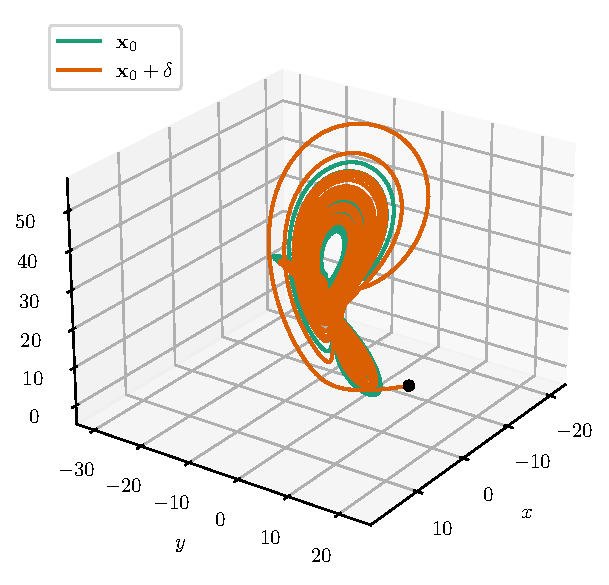
\includegraphics[width=0.7\textwidth]{figs/ode/lorenz_sensitivity.pdf}
        \caption{Sensitivity in the Lorenz system. Two trajectories are integrated from nearly identical initial conditions, differing only in the $z$ component by $10^{-4}$. Although they initially track each other closely, they eventually diverge. This shows the extreme sensitivity to initial conditions that makes standard shooting methods unstable over long time intervals for chaotic systems.}
        \label{fig:lorenz}
    \end{figure}
\end{exampleBox}

\paragraph*{The Multiple Shooting Method}

To mitigate the sensitivity problem, we can use the multiple shooting method. The idea is to break the long integration interval $[0, T]$ into $M$ smaller sub-intervals. That is, we partition the interval as $0 = t_0 < t_1 < \dots < t_M = T$, where $t_i = i\Delta t$ (\autoref{fig:multiple_shooting_diagram}). For each sub-interval $[t_i, t_{i+1}]$, we introduce an unknown initial state $\mathbf{c}_i \approx \mathbf{x}(t_i)$ and define the local solution $\mathbf{x}_i(t)$ as the solution of:
\begin{equation}
    \dot{\mathbf{x}}_i = \mathbf{f}(\mathbf{x}_i, t), \quad \mathbf{x}_i(t_i) = \mathbf{c}_i, \quad t \in [t_i, t_{i+1}]
\end{equation}
To make sure these separate pieces form a valid continuous solution for the original BVP, we impose continuity constraints at the nodes such that the end of one interval matches the start of the next.
\begin{equation}
    \mathbf{x}_i(t_{i+1}) - \mathbf{c}_{i+1} = \mathbf{0}, \quad i = 0, \dots, M-2
\end{equation}
Combined with the boundary conditions (which now map the very first $\mathbf{c}_0$ and the very last $\mathbf{x}_{M-1}(t_M)$), we now have a system of equations in $N \cdot M$ unknowns. In practice, this large nonlinear system is solved by Newton's method. The Jacobian has a sparse block structure due to the local coupling between neighboring intervals. By keeping the sub-intervals short, we prevent the sensitivity matrix $\mathbf{S}$ from growing exponentially large within any single step and keep the condition number manageable.

\begin{figure}[H]
    % MC: I think this figure is a little confusing w.r.t. what's actually going on in the multiple shooting method, but I'll leave it for now since it matches the slides
    % it seems to imply that the solution is piecewise linear, but it's not necessarily the case
    \centering
    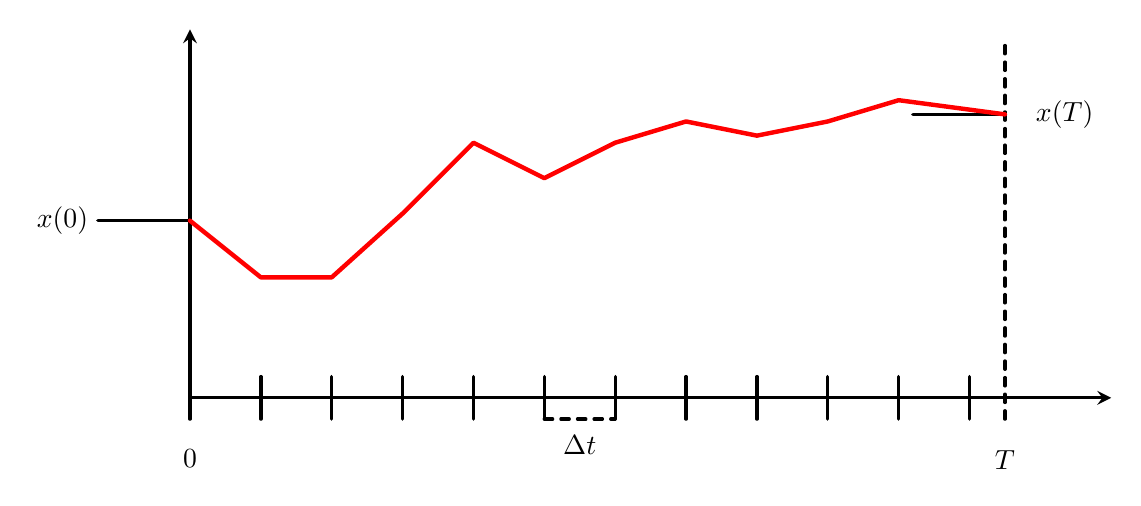
\begin{tikzpicture}[
        scale=0.9,
        >=stealth,
        line cap=round,
        line join=round
    ]
    % TODO: should add initial conditions of each interval to show setup explicitly
        % axes
        \draw[very thick,->] (0,-.3) -- (0,5.2);
        \draw[very thick,->] (0,0)     -- (13,0);

        % time ticks
        \foreach \x in {1,...,11}{
        \draw[very thick] (\x,0.3) -- (\x,-0.3);
        }

        % dashed line at T
        \draw[very thick,dashed] (11.5,-.3) -- (11.5,5.0);

        % horizontal levels x(0) and x(T)
        \draw[very thick] (-1.3,2.5) -- (0,2.5);      % x(0)
        \draw[very thick] (10.2,4.0) -- (11.5,4.0);   % x(T)

        % sample path
        \draw[ultra thick,red]
        (0,2.5)  --
        (1,1.7)  --
        (2,1.7)  --
        (3,2.6)  --
        (4,3.6)  --
        (5,3.1)  --
        (6,3.6)  --
        (7,3.9)  --
        (8,3.7)  --
        (9,3.9)  --
        (10,4.2) --
        (11.5,4.0);

        \draw[very thick,dashed] (5,-0.3) -- (6,-0.3);

        \node[below] at (0,-.6) {$0$};
        \node[below] at (11.5,-.6) {$T$};
        \node[below] at (5.5,-.4) {$\Delta t$};

        \node[left]  at (-1.3,2.5) {$x(0)$};
        \node[right] at (11.8,4.0) {$x(T)$};

    \end{tikzpicture}
    \caption{Schematic of the multiple shooting method. The long interval $[0,T]$ is partitioned into $M$ sub-intervals $[t_i,t_{i+1}]$ with $t_i = i\Delta t$. On each sub-interval, a local trajectory $\mathbf{x}_i(t)$ is integrated from an independent initial value $\mathbf{c}_i \approx \mathbf{x}(t_i)$. Continuity constraints enforce that the end point of one segment matches the initial value of the next, $\mathbf{x}_i(t_{i+1}) = \mathbf{c}_{i+1}$, so that the segments form a single continuous solution of the BVP. Note that the solution is not necessarily piecewise linear (it just is for the case shown here).}
    \label{fig:multiple_shooting_diagram}
\end{figure}

\section{Discretization Methods}

\subsection{The Finite Difference Method}

We can arrive at a powerful alternative to shooting methods by taking the concept of multiple shooting to its logical limit. Recall that in multiple shooting, we divided the domain $[0, T]$ into $M$ sub-intervals and solved an IVP over each small segment $[t_i, t_{i+1}]$. We then glued these solutions together by enforcing continuity $\mathbf{x}(t_{i+1}; \mathbf{c}_i) = \mathbf{c}_{i+1}$. Now, imagine we decrease the interval size $\Delta t$ until it is so small that a single step of the simplest explicit Euler method is sufficiently accurate to represent the ODE dynamics. In this limit, the condition that the solution at the end of interval $i$ matches the start of interval $i+1$ becomes a simple algebraic relationship:
\begin{equation}
    \mathbf{c}_{i+1} = \mathbf{c}_i + \Delta t \, \mathbf{f}(\mathbf{c}_i, t_i)
\end{equation}
This equation relates the values of the solution at adjacent grid points directly without needing to run an ODE solver. If we rearrange this, we see that it effectively approximates the derivative using the slope between points. This viewpoint is what motivates finite differences. Instead of integrating the differential equation, we discretize the differential operator itself. We replace the continuous domain with a discrete grid of $M+1$ points (nodes) and replace the derivatives in the differential equation with algebraic difference quotients involving the values at these nodes. This converts the BVP into a large system of coupled nonlinear algebraic equations, which we can solve using Newton's method.

\begin{figure}[H]
    \centering
    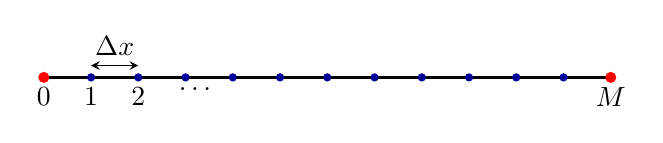
\begin{tikzpicture}[>=stealth]

    % parameters
    \def\M{12}        % number of intervals
    \def\dx{0.6}      % spacing between grid points

    % horizontal line
    \draw[thick] (0,0) -- (\M*\dx,0);

    % interior grid points (blue)
    \foreach \k in {1,...,\numexpr\M-1\relax}{
    \fill[blue!60!black] (\k*\dx,0) circle (1.5pt);
    }

    % boundary grid points (red)
    \fill[red] (0,0) circle (2pt);
    \fill[red] (\M*\dx,0) circle (2pt);

    % labels x=0 and x=1
    % \node[above] at (0,0.05) {$x=0$};
    % \node[above] at (\M*\dx,0.05) {$x=1$};

    % index labels
    \node[below] at (0,0) {$0$};
    \node[below] at (\dx,0) {$1$};
    \node[below] at (2*\dx,0) {$2$};
    \node[below] at (3.2*\dx,0) {$\dots$};
    \node[below] at (\M*\dx,0) {$M$};

    % Delta x arrow
    \draw[<->] (\dx,0.15) -- (2*\dx,0.15);
    \node[above] at (1.5*\dx,0.15) {$\Delta x$};

    \end{tikzpicture}
    \caption{Discretization of the domain into $M$ intervals of width $\Delta x$.}
    \label{fig:finite_difference_diagram}
\end{figure}


\paragraph*{Finite Difference Approximations}

To formalize this, we define a grid $x_m = x_0 + m\Delta x$ for $m=0, 1, \dots, M$, where $\Delta x$ is the grid spacing. We seek approximate values $C_m \approx c(x_m)$. We approximate the derivatives $f^{(p)}(x)$ at a node using a weighted sum of function values at neighboring nodes:
\begin{equation}
    f^{(p)}(x_0) \approx \frac{1}{(\Delta x)^p} \sum_{m} \alpha_m f(x_m)
\end{equation}
We can derive these coefficients $\alpha_m$ and analyze their accuracy using Taylor series expansions. For the first derivative $f'(x)$, a symmetric \textbf{central difference} uses the points immediately to the left and right:
\begin{equation}
    f'(x) \approx \frac{f(x + \Delta x) - f(x - \Delta x)}{2\Delta x}
\end{equation}
By expanding $f(x+\Delta x)$ and $f(x-\Delta x)$ in Taylor series up to the third order and subtracting them, terms involving $f(x)$ and $f''(x)$ cancel out, leaving the first derivative term plus an error term proportional to $(\Delta x)^2 f'''(x)$. Thus, this approximation is \textit{second-order accurate}, or $O(\Delta x^2)$.

For the second derivative $f''(x)$, which appears frequently in diffusion and wave problems, we combine the values at $x-\Delta x$, $x$, and $x+\Delta x$:
\begin{equation}
    f''(x) \approx \frac{f(x - \Delta x) - 2f(x) + f(x + \Delta x)}{(\Delta x)^2}
\end{equation}
Again, Taylor analysis confirms this approximation is second-order accurate. Specifically, the error term scales with $(\Delta x)^2 f^{(4)}(x)$. High-order accuracy is desirable because it implies that refining the grid (reducing $\Delta x$) leads to a rapid reduction in numerical error.

\paragraph*{Application: Reaction-Diffusion System}

Let us apply this method to the concrete physical example of a steady-state reaction-diffusion system in a 1D slab. The governing equation is
\begin{equation}
    \frac{d^2 c}{dx^2} = -r(c)
\end{equation}
where $c(x)$ is the concentration and $r(c)$ is the reaction rate. The domain is $x \in [0, 1]$. We impose generalized Robin boundary conditions at both ends, which relate the concentration and its flux:
\begin{align}
    x=0: & \quad A_0 \frac{dc}{dx} + B_0 c = C_0 \\
    x=1: & \quad A_1 \frac{dc}{dx} + B_1 c = C_1
\end{align}
We discretize the domain into $M$ intervals of size $\Delta x = 1/M$, creating $M+1$ unknown variables $c_0, c_1, \dots, c_M$. For every interior node $m = 1, \dots, M-1$, we replace the second derivative with the central difference approximation derived above. Substituting this into the ODE produces one algebraic equation per node:
\begin{equation}
    \frac{1}{(\Delta x)^2} (c_{m-1} - 2c_m + c_{m+1}) + r(c_m) = 0
\end{equation}
This provides $M-1$ equations for our $M+1$ unknowns. To close the system, we must derive equations for the two boundary nodes $m=0$ and $m=M$ using the boundary conditions. The boundary conditions involve the first derivative $dc/dx$. We must approximate this derivative using the available grid points. At the left boundary ($x=0$, node $m=0$), we cannot use a central difference because there is no node at $x_{-1}$. Instead, we can use a forward difference. A simple first-order forward difference is $(c_1 - c_0)/\Delta x$. However, since our interior scheme is second-order accurate ($O(\Delta x^2)$), using a first-order boundary approximation ($O(\Delta x)$) would degrade the global accuracy of the solution. To maintain second-order accuracy, we employ a three-point forward difference approximation for the derivative at the boundary. The boundary equation at $x=0$ becomes
\begin{equation}
    g_0(\mathbf{c}) = A_0 \left[ \frac{-3c_0 + 4c_1 - c_2}{2\Delta x} \right] + B_0 c_0 - C_0 = 0
\end{equation}
Similarly, at the right boundary ($x=1$, node $m=M$), we use a three-point backward difference:
\begin{equation}
    g_M(\mathbf{c}) = A_1 \left[ \frac{3c_M - 4c_{M-1} + c_{M-2}}{2\Delta x} \right] + B_1 c_M - C_1 = 0
\end{equation}
(Note: these three-point formulas require $M \ge 2$ so that the necessary interior points exist.) Collecting the equations for the boundaries and the interior points, we obtain a system of $M+1$ nonlinear algebraic equations for the $M+1$ unknowns. We define the residual vector function $\mathbf{G}(\mathbf{c}) = \mathbf{0}$, where
\begin{equation}
    \mathbf{G}(\mathbf{c}) = \begin{bmatrix}
        g_0(\mathbf{c}) \\
        \frac{1}{(\Delta x)^2} (c_0 - 2c_1 + c_2) + r(c_1) \\
        \vdots \\
        \frac{1}{(\Delta x)^2} (c_{M-2} - 2c_{M-1} + c_M) + r(c_{M-1}) \\
        g_M(\mathbf{c})
    \end{bmatrix} = \mathbf{0}
\end{equation}
This system is usually sparse and structured (tridiagonal or pentadiagonal), which makes it computationally efficient to solve using Newton-Raphson methods, such as \texttt{fsolve} in MATLAB or \texttt{scipy.optimize.root} in Python.

\begin{figure}[H]
    \centering
    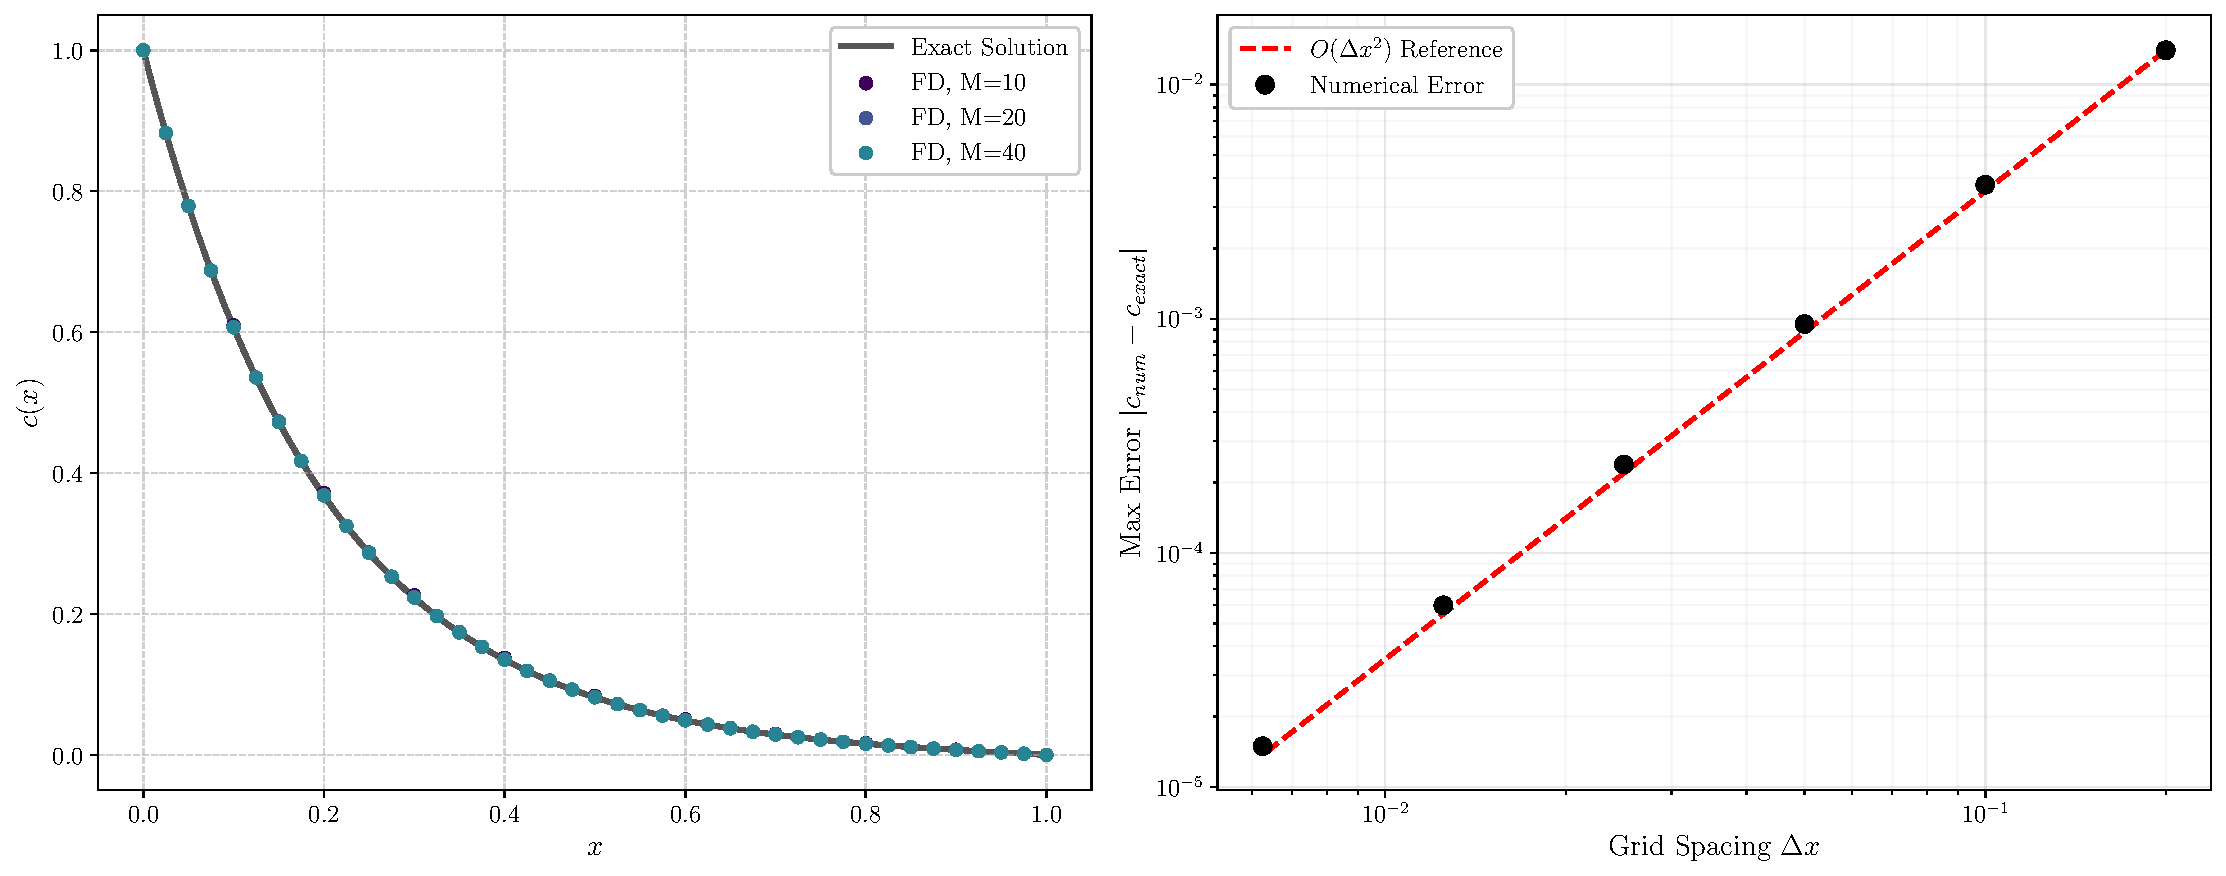
\includegraphics[width=0.95\textwidth]{figs/ode/finite_difference_convergence.pdf}
    \caption{Finite difference solution and convergence analysis. Left: Numerical solutions for the reaction-diffusion problem ($c'' = -kc$ with boundary conditions $c(0)=1, c(1)=0$) using varying grid resolutions ($M=10, 20, 40$) compared to the exact analytical solution (solid gray line). Right: Log-log convergence plot showing the maximum error between the numerical and exact solutions versus the grid spacing $\Delta x$. The error data points (black dots) align almost perfectly with the red dashed reference line representing quadratic scaling, which confirms the theoretical $O(\Delta x^2)$ accuracy of the central difference scheme.}
    \label{fig:fd_convergence}
\end{figure}

The accuracy of the numerical solution depends heavily on the grid spacing. As shown in \autoref{fig:fd_convergence}, a plot of the error against the grid spacing $\Delta x$ on a logarithmic scale has a slope of 2. This empirically verifies that our choice of central differences for the interior and three-point differences for the boundaries gives a globally second-order accurate solution. While the finite difference method requires solving a large simultaneous system (unlike the shooting method, which solves small IVPs sequentially), it is generally more robust and less sensitive to initial guesses, particularly for stiff or unstable differential equations.

\paragraph*{Accuracy Analysis of Finite Differences}

To justify the accuracy of the finite difference approximations used in the previous section, we use Taylor's theorem. This allows us to quantify the local truncation error introduced by discretizing the continuous differential operator. Consider the central difference approximation for the first derivative. We expand the function values at the neighboring nodes $x + \Delta x$ and $x - \Delta x$ around the central point $x$:
\begin{align}
    f(x + \Delta x) &= f(x) + \Delta x f'(x) + \frac{(\Delta x)^2}{2} f''(x) + \frac{(\Delta x)^3}{6} f'''(x) + O(\Delta x^4) \\
    f(x - \Delta x) &= f(x) - \Delta x f'(x) + \frac{(\Delta x)^2}{2} f''(x) - \frac{(\Delta x)^3}{6} f'''(x) + O(\Delta x^4)
\end{align}
Subtracting the second equation from the first causes the even-order derivative terms to cancel out. We are left with the difference $f(x + \Delta x) - f(x - \Delta x) = 2\Delta x f'(x) + \frac{(\Delta x)^3}{3} f'''(x) + \dots$. Dividing by $2\Delta x$ isolates the first derivative:
\begin{equation}
    \frac{f(x + \Delta x) - f(x - \Delta x)}{2\Delta x} = f'(x) + \frac{(\Delta x)^2}{6} f'''(x) + \dots
\end{equation}
The dominant error term is proportional to $(\Delta x)^2$. Consequently, we say this approximation is second-order accurate, or $O(\Delta x^2)$. A similar procedure for the second derivative approximation $f''(x) \approx (f(x+\Delta x) - 2f(x) + f(x-\Delta x))/(\Delta x)^2$ also yields an error term proportional to $(\Delta x)^2 f^{(4)}(x)$, confirming that the standard central difference scheme maintains second-order consistency throughout the domain.

\paragraph*{Relation to Multiple Shooting}

We've mentioned this before, but it is instructive to recognize that the finite difference method is not entirely distinct from the shooting methods discussed earlier; rather, it is a limiting case. Recall that in the multiple shooting method, we partition the domain $[0, T]$ into $M$ sub-intervals and solve an IVP on each segment, enforcing continuity $\mathbf{c}_{i} = \mathbf{x}(t_i; \mathbf{c}_{i-1})$ at the nodes. If we decrease the interval size $\Delta t$ until it is small enough that a single step of an explicit Euler integrator is sufficient, the continuity condition simplifies. The integration step becomes $\mathbf{c}_i = \mathbf{c}_{i-1} + \Delta t \, \mathbf{f}(\mathbf{c}_{i-1}, t_{i-1})$. Rearranging this yields $(\mathbf{c}_i - \mathbf{c}_{i-1})/\Delta t = \mathbf{f}(\mathbf{c}_{i-1})$, which is exactly the finite difference formulation using a forward difference. Thus, we can view the finite difference method as a multiple shooting method where the number of intervals $M$ approaches the number of grid points, and the ``shooting'' (IVP integration) is replaced by a simple algebraic step. The resulting system of nonlinear equations involves $(M+1)N$ variables and equations, which can be solved simultaneously using Newton-Raphson.

\subsection{Basis Function Expansions}

Basis function expansion methods (also called spectral methods or weighted residual methods) take a different approach than the grid-discretization methods discussed above. We approximate the solution $c(x)$ as a continuous function constructed from a linear combination of pre-selected basis functions $\{\Phi_j(x)\}_{j=1}^M$. The approximate solution is written as
\begin{equation}
    c(x) \approx \sum_{j=1}^M c_j \Phi_j(x)
\end{equation}
The problem of solving the differential equation is thus transformed into the problem of finding the optimal set of scalar coefficients $c_1, \dots, c_M$. This approach is powerful because, with a wise choice of basis functions (such as orthogonal polynomials or Fourier modes), we can achieve high accuracy with relatively few coefficients.

\paragraph*{Handling Boundary Conditions}

Before determining the coefficients, we must ensure the boundary conditions are satisfied. Consider a general BVP with Dirichlet boundary conditions:
\begin{equation}
    \frac{d^2c}{dx^2} = f(x), \quad c(0) = a, \quad c(1) = b
    \label{eq:bvp-dirichlet}
\end{equation}
If our basis functions are arbitrary, satisfying $c(0)=a$ and $c(1)=b$ constrains the coefficients $c_j$ in a complicated way. To simplify this, we use a splitting technique. We assume the solution can be decomposed into a particular function $c_p(x)$ and a homogeneous function $c_h(x)$:
\begin{equation}
    c(x) = c_p(x) + c_h(x)
\end{equation}
The particular function $c_p(x)$ is chosen solely to satisfy the boundary conditions. For instance, the linear function $c_p(x) = a + (b-a)x$ satisfies $c_p(0)=a$ and $c_p(1)=b$. The remaining part, $c_h(x)$, must then satisfy homogeneous boundary conditions ($c_h(0)=0, c_h(1)=0$) so that the sum matches the original BCs. By substituting this decomposition into the original ODE, we get a new differential equation for $c_h(x)$ where the forcing term is modified by derivatives of $c_p(x)$ but the boundary conditions are strictly zero. Without loss of generality, we can therefore restrict our study to BVPs with homogeneous boundary conditions. We choose basis functions $\{\Phi_j(x)\}$ that individually satisfy $\Phi_j(0) = 0$ and $\Phi_j(1) = 0$. Consequently, any linear combination of these functions automatically satisfies the boundary conditions, allowing us to focus entirely on satisfying the differential equation inside the domain.

\paragraph*{Weighted Residuals}

We substitute our expansion $c(x) = \sum c_j \Phi_j(x)$ into the differential equation $c'' - f(x) = 0$ (\autoref{eq:bvp-dirichlet}). Since our approximation is not exact, this substitution produces a non-zero residual function $R(x; \mathbf{c})$:
\begin{equation}
    R(x; \mathbf{c}) = \sum_{j=1}^M c_j \Phi_j''(x) - f(x) \neq 0
\end{equation}
We cannot force the residual to be zero everywhere (that would require the exact solution). Instead, we enforce that the residual is zero in a weighted average sense. We introduce a set of test functions (or weight functions) $\{\Psi_i(x)\}_{i=1}^M$ and require the integral of the residual against each test function to vanish:
\begin{equation}
    \int_0^1 \Psi_i(x) R(x; \mathbf{c}) \, dx = 0, \quad \text{for } i = 1, \dots, M
\end{equation}
Expanding this integral, we get a system of linear equations for the coefficients $c_j$:
\begin{equation}
    \sum_{j=1}^M c_j \left( \int_0^1 \Psi_i(x) \Phi_j''(x) \, dx \right) = \int_0^1 \Psi_i(x) f(x) \, dx
\end{equation}
This can be written as a matrix system $\mathbf{A}\mathbf{c} = \mathbf{b}$. The choice of the test functions $\{\Psi_i(x)\}$ determines the specific numerical method. Two such choices are the collocation method and the Galerkin method.

\paragraph*{The Collocation Method}

In the collocation method, we choose the test functions to be Dirac delta functions centered at specific points $x_i$: $\Psi_i(x) = \delta(x - x_i)$. The integral property of the delta function sifts out the value of the residual at $x_i$. Physically, this implies we are forcing the differential equation to hold exactly at a set of $M$ discrete collocation points $\{x_i\}_{i=1}^M$. The equations become
\begin{equation}
    \sum_{j=1}^M c_j \Phi_j''(x_i) = f(x_i), \quad \text{for } i = 1, \dots, M
\end{equation}
Usually, the collocation points are chosen to be the roots of orthogonal polynomials (such as Legendre polynomials) to minimize the error between points, a technique known as orthogonal collocation.

\paragraph*{The Galerkin Method}

In the Galerkin method, we choose the test functions to be the same as the basis functions: $\Psi_i(x) = \Phi_i(x)$. We are basically projecting the residual onto the space spanned by the basis functions and demanding that the error is orthogonal to our approximation space. The condition is
\begin{equation}
    \sum_{j=1}^M c_j \left( \int_0^1 \Phi_i(x) \Phi_j''(x) \, dx \right) = \int_0^1 \Phi_i(x) f(x) \, dx
\end{equation}
If the basis functions $\{\Phi_j(x)\}$ are eigenfunctions of the differential operator (e.g., $\Phi_j'' = \lambda_j \Phi_j$) and are orthogonal (meaning $\int \Phi_i \Phi_j dx = 0$ for $i \neq j$), the matrix on the left-hand side becomes diagonal or highly structured, making the system trivial to solve.

\begin{exampleBox}
    \textbf{Example: Solving a BVP with Basis Functions}
    
    Consider the following BVP:
    \begin{equation}
        \frac{d^2c}{dx^2} - c = \exp(-x^2), \quad c(0) = c(1) = 0
    \end{equation}
    Since the boundary conditions are homogeneous and Dirichlet, a natural choice for basis functions are the sine modes, which are eigenfunctions of the second derivative operator:
    \begin{equation}
        \Phi_j(x) = \sin(j \pi x), \quad j=1, \dots, M
    \end{equation}
    These functions satisfy $\Phi_j(0)=\Phi_j(1)=0$ automatically. We seek $c(x) = \sum c_j \sin(j \pi x)$.
    
    \textbf{1. Collocation Approach:}
    We choose $M$ points $x_i$ evenly spaced in $(0, 1)$. We substitute the sum into the ODE ($c'' - c$) and evaluate at each $x_i$:
    \begin{equation}
        \sum_{j=1}^M c_j \left[ -(j\pi)^2 \sin(j\pi x_i) - \sin(j\pi x_i) \right] = \exp(-x_i^2)
    \end{equation}
    This is a linear system $\mathbf{A}\mathbf{c} = \mathbf{b}$ where $A_{ij} = -((j\pi)^2 + 1)\sin(j\pi x_i)$.
    
    \textbf{2. Galerkin Approach:}
    We multiply the residual by $\Phi_i(x) = \sin(i \pi x)$ and integrate from 0 to 1. Due to the orthogonality of sines, the cross terms in the sum vanish ($\int \sin(i\pi x)\sin(j\pi x) dx = 0$ for $i \neq j$). The term involving the second derivative becomes:
    \begin{equation}
        \int_0^1 \sin(i \pi x) \frac{d^2}{dx^2} \left( c_i \sin(i \pi x) \right) dx = -c_i (i\pi)^2 \int_0^1 \sin^2(i \pi x) dx = -c_i \frac{(i\pi)^2}{2}
    \end{equation}
    Similarly, the term $\int c \Phi_i dx$ yields $c_i/2$. The equation for coefficient $c_i$ decouples completely:
    \begin{equation}
        -\frac{1}{2} \left[ (i\pi)^2 + 1 \right] c_i = \int_0^1 \exp(-x^2) \sin(i \pi x) dx
    \end{equation}
    We can calculate the integral on the right-hand side (numerically or analytically) and directly divide by the scalar factor $-\frac{1}{2}[(i\pi)^2 + 1]$ to find each $c_i$.
    
    \begin{figure}[H]
        \centering
        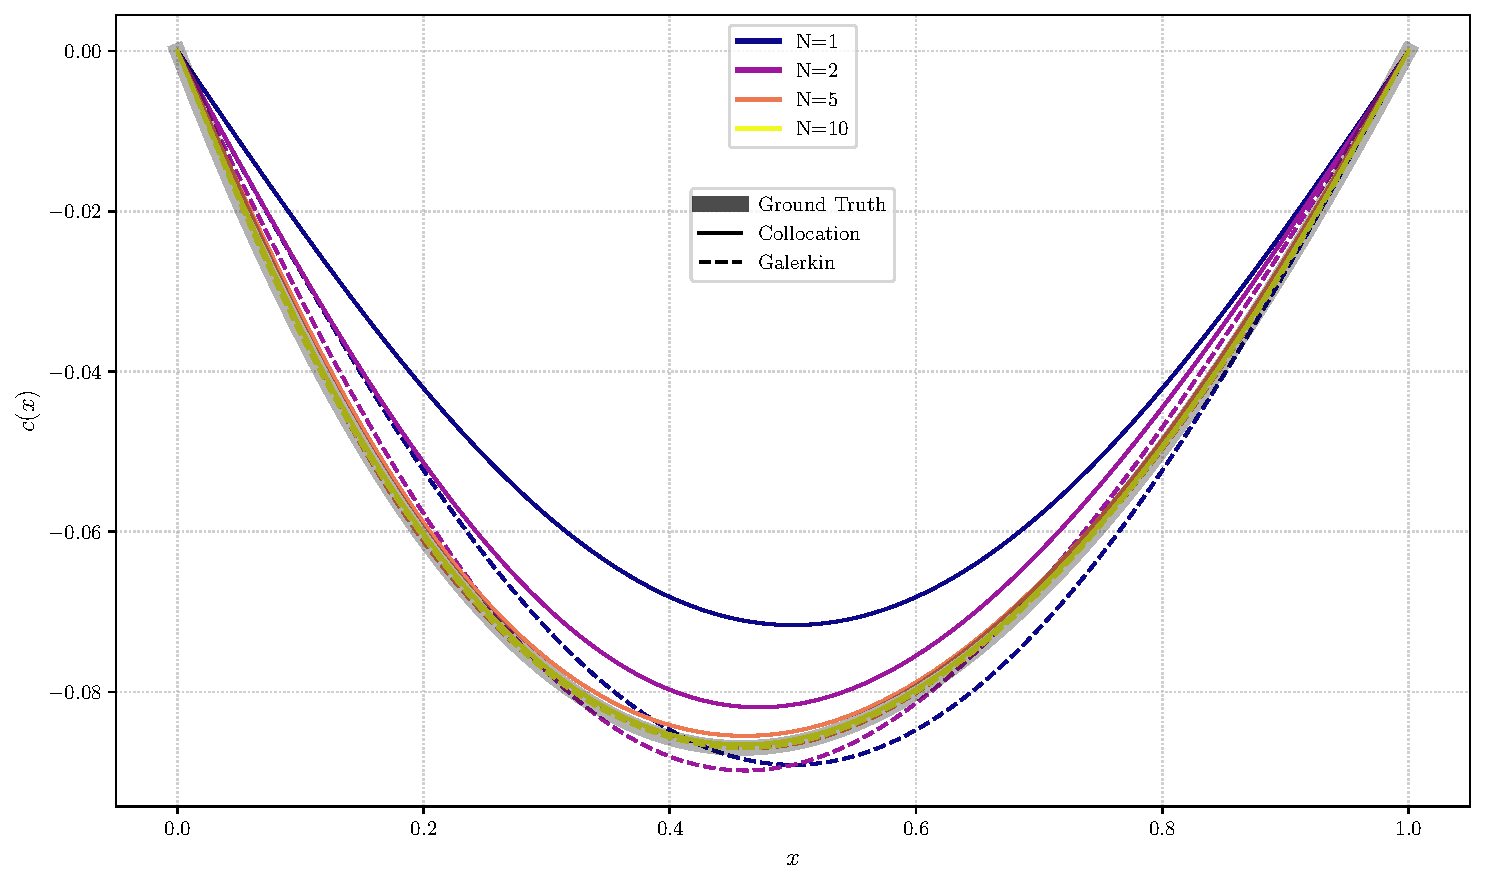
\includegraphics[width=0.6\textwidth]{figs/ode/bvp_coll_galerkin.pdf}
        \caption{Comparison of collocation and Galerkin methods for the example BVP. As the number of basis functions $N$ increases (colored lines), both methods converge to the true solution (gray band). The Galerkin method minimizes the global integrated error, while collocation drives the error to zero specifically at the chosen points.}
        \label{fig:bvp_coll_galerkin}
    \end{figure}
\end{exampleBox}

\subsection{The Finite Element Method}

The basis function expansion methods discussed previously, particularly when using global polynomials or eigenfunctions (like sine waves), have a significant computational issue. This issue is that these functions are global; that is, they are non-zero over the entire domain. Consequently, when we compute the inner products for the Galerkin method, every basis function interacts with every other basis function. This results in a dense system matrix $\mathbf{A}$, where every entry is potentially non-zero. Solving a dense linear system requires $O(M^3)$ operations, which becomes prohibitively expensive as the number of modes $M$ increases. Furthermore, finding suitable global basis functions for complex, irregular geometries is often impossible.

To overcome these limitations, we introduce the \textbf{finite element method (FEM)}. The philosophy of FEM is to retain the integral formulation of the Galerkin method but to replace the global basis functions with \textit{local} basis functions.

\paragraph*{Local Basis Functions}

We partition the domain $[0, 1]$ into a grid of nodes $x_0, x_1, \dots, x_M$, similar to the finite difference grid. However, instead of approximating the derivative at a point, we define basis functions $\Phi_m(x)$ that are non-zero only over a small sub-interval around node $x_m$. The simplest choice is the piecewise linear ``hat'' or ``tent'' function defined as:
\begin{equation}
    \Phi_m(x) = \begin{cases} 
      \frac{x - x_{m-1}}{\Delta x} & x_{m-1} < x \le x_m \\
      \frac{x_{m+1} - x}{\Delta x} & x_m < x < x_{m+1} \\
      0 & \text{otherwise} 
   \end{cases}
\end{equation}
where $\Delta x$ is the spacing between nodes. Each function $\Phi_m(x)$ rises linearly from 0 to 1 and falls back to 0 over a span of $2\Delta x$. Taking linear combinations of these local tent functions allows us to construct a global piecewise-linear approximation of any given function. Importantly, $\Phi_i(x)$ and $\Phi_j(x)$ have no overlap if $|i - j| > 1$. This locality property guarantees that the vast majority of integrals in the Galerkin formulation will be zero, leading to a sparse, banded matrix that is computationally efficient to solve.

\begin{figure}[H]
    \centering
    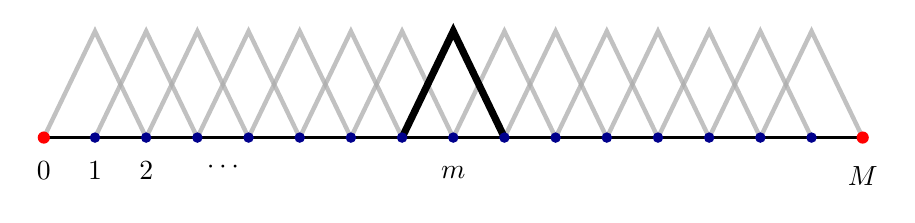
\begin{tikzpicture}[x=0.65cm,y=1cm]
    % parameters
    \def\M{16}   % right endpoint index (labeled M)
    \def\m{8}    % highlighted index (labeled m)
    \def\H{1.35} % hat height

    \pgfmathtruncatemacro{\Mminusone}{\M-1}

    % baseline
    \draw[line width=1.2pt] (0,0) -- (\M,0);

    % grey hat functions (all i = 1,...,M-1)
    \foreach \i in {1,...,\Mminusone}{
        \draw[gray!65,opacity=0.75,line width=1.6pt,line cap=round]
        ({\i-1},0) -- (\i,\H) -- ({\i+1},0);
    }

    % highlighted hat at i = m
    \draw[black,line width=2.6pt,line cap=round]
        ({\m-1},0) -- (\m,\H) -- ({\m+1},0);

    % nodes on the line
    \fill[red] (0,0) circle (2.2pt);
    \fill[red] (\M,0) circle (2.2pt);
    \foreach \i in {1,...,\Mminusone}{
        \fill[blue!55!black] (\i,0) circle (1.9pt);
    }

    % labels
    % \node[left=10pt]  at (0,0)  {$x=0$};
    % \node[right=10pt] at (\M,0) {$x=1$};

    \node[below=5pt] at (0,0) {$0$};
    \node[below=5pt] at (1,0) {$1$};
    \node[below=5pt] at (2,0) {$2$};
    \node[below=5pt] at (3.5,0) {$\cdots$};
    \node[below=7pt] at (\m,0) {$m$};
    \node[below=7pt] at (\M,0) {$M$};
    \end{tikzpicture}
    \caption{Local tent basis functions for the FEM.}
    \label{fig:fem_basis}
\end{figure}

\paragraph*{The Weak Formulation}

Let us apply this to our model problem:
\begin{equation}
    \frac{d^2c}{dx^2} - c = \exp(-x^2), \quad c(0)=0, \quad c(1)=0
\end{equation}
We approximate the solution as a linear combination of these tent functions: $c(x) \approx \sum_{j=1}^{M-1} c_j \Phi_j(x)$. Note that we exclude $j=0$ and $j=M$ from the unknowns because the boundary conditions $c(0)=0$ and $c(1)=0$ fix those coefficients to zero. We now plug this approximation into the Galerkin condition. If we tried to do this in the ``strong'' form, i.e.,
\begin{equation}
    \int_0^1 \bigl(c_h''(x) - c_h(x) - f(x)\bigr)\,\Phi_i(x)\,dx = 0
\end{equation}
we immediately run into the issue that since $\Phi_j$ is only piecewise linear, $\Phi_j'$ is piecewise constant and $\Phi_j''$ is not an ordinary function at all (it lives at the nodes as delta spikes). Considering this, the standard FEM trick is to integrate by parts once so that we only need first derivatives. Concretely,
\begin{equation}
    \int_0^1 c_h''(x)\,\Phi_i(x)\,dx
    = \Bigl[c_h'(x)\,\Phi_i(x)\Bigr]_{0}^{1} - \int_0^1 c_h'(x)\,\Phi_i'(x)\,dx
\end{equation}
For interior test functions $i=1,\dots,M-1$, the hats satisfy $\Phi_i(0)=\Phi_i(1)=0$, so the boundary term drops:
\begin{equation}
    \Bigl[c_h'(x)\,\Phi_i(x)\Bigr]_{0}^{1} = 0
\end{equation}
So the weak (integrated-by-parts) Galerkin equations become
\begin{equation}
    -\int_0^1 c_h'(x)\,\Phi_i'(x)\,dx - \int_0^1 c_h(x)\,\Phi_i(x)\,dx
    = \int_0^1 f(x)\,\Phi_i(x)\,dx
    \qquad i=1,\dots,M-1
\end{equation}
where here $f(x)=e^{-x^2}$. Now, we substitute the expansion $c_h=\sum_{j=1}^{M-1}c_j\Phi_j$ and pull the coefficients $c_j$ outside the integrals:
\begin{equation}
    \sum_{j=1}^{M-1} c_j\left(
        -\int_0^1 \Phi_j'(x)\,\Phi_i'(x)\,dx
        -
        \int_0^1 \Phi_j(x)\,\Phi_i(x)\,dx
    \right)
    = \int_0^1 f(x)\,\Phi_i(x)\,dx
\end{equation}
At this point, it is helpful to name the two standard FEM matrices. The derivative term is the \emph{stiffness} matrix,
\begin{equation}
    K_{ij} = \int_0^1 \Phi_j'(x)\,\Phi_i'(x)\,dx
\end{equation}
and the term with the functions themselves is the \emph{mass} matrix,
\begin{equation}
    M_{ij} = \int_0^1 \Phi_j(x)\,\Phi_i(x)\,dx
\end{equation}
The right-hand side is just the load vector entry
\begin{equation}
    b_i = \int_0^1 f(x)\,\Phi_i(x)\,dx
\end{equation}
With this notation, the linear system is simply
\begin{equation}
    \sum_{j=1}^{M-1}\bigl(-K_{ij}-M_{ij}\bigr)c_j = b_i
    \qquad i=1,\dots,M-1,
\end{equation}
or, in matrix form, $\mathbf{A}\mathbf{c}=\mathbf{b}$ with $A_{ij}=-K_{ij}-M_{ij}$. (Note that since our operator is formally $d^2/dx^2 - I$, which is negative definite, the matrix $\mathbf{A}$ is negative definite. In many texts, the problem is multiplied by $-1$ to yield a positive-definite system $(K+M)\mathbf{c} = -\mathbf{b}$. Just be aware of this.) The big practical win here is sparsity: each hat $\Phi_i$ only overlaps with $\Phi_{i-1}$ and $\Phi_{i+1}$, so
\begin{equation}
    K_{ij}=M_{ij}=0\qquad\text{whenever}\qquad |i-j|>1
\end{equation}
meaning $\mathbf{A}$ is tridiagonal. On a uniform grid with spacing $\Delta x$, the stiffness entries come straight from the fact that $\Phi_i'$ is $\frac{1}{\Delta x}$ on the left element and $-\frac{1}{\Delta x}$ on the right element. For the diagonal,
\begin{equation}
    K_{ii}
    = \int_{x_{i-1}}^{x_i}\left(\frac{1}{\Delta x}\right)^2 dx
      + \int_{x_i}^{x_{i+1}}\left(-\frac{1}{\Delta x}\right)^2 dx
    = \frac{2}{\Delta x}
\end{equation}
and for the neighbors (say $i$ and $i+1$), the derivatives have opposite signs on the shared element $[x_i,x_{i+1}]$, giving
\begin{equation}
    K_{i,i+1}
    = \int_{x_i}^{x_{i+1}}\left(-\frac{1}{\Delta x}\right)\left(\frac{1}{\Delta x}\right)\,dx
    = -\frac{1}{\Delta x}
\end{equation}
and similarly $K_{i,i-1}=-\frac{1}{\Delta x}$. For the mass matrix, you can either do the little triangles-by-hand integrals or just remember the standard results for linear elements. The diagonal is
\begin{equation}
    M_{ii} = \int_0^1 \Phi_i(x)^2\,dx = \frac{2}{3}\Delta x,
\end{equation}
and the off-diagonal neighbor coupling is
\begin{equation}
    M_{i,i+1} = \int_0^1 \Phi_i(x)\,\Phi_{i+1}(x)\,dx = \frac{1}{6}\Delta x
\end{equation}
with the same value for $M_{i,i-1}$. Putting these together, the $i$th row of the FEM system (only involving $c_{i-1},c_i,c_{i+1}$) reads
\begin{equation}
    -\Bigl(K_{i,i-1}c_{i-1}+K_{ii}c_i+K_{i,i+1}c_{i+1}\Bigr)
    -\Bigl(M_{i,i-1}c_{i-1}+M_{ii}c_i+M_{i,i+1}c_{i+1}\Bigr)
    = b_i,
\end{equation}
i.e.,
\begin{equation}
    -\left(-\frac{1}{\Delta x}c_{i-1} + \frac{2}{\Delta x}c_i - \frac{1}{\Delta x}c_{i+1}\right)
    -\left(\frac{\Delta x}{6}c_{i-1} + \frac{2\Delta x}{3}c_i + \frac{\Delta x}{6}c_{i+1}\right)
    = \int_0^1 e^{-x^2}\,\Phi_i(x)\,dx
\end{equation}
If we group the terms in the nicer ``stencil'' form, we get
\begin{equation}
    \frac{1}{\Delta x}\bigl(c_{i-1}-2c_i+c_{i+1}\bigr)
    -
    \frac{\Delta x}{6}\bigl(c_{i-1}+4c_i+c_{i+1}\bigr)
    =
    \int_0^1 e^{-x^2}\,\Phi_i(x)\,dx
\end{equation}
This system is tridiagonal and sparse, so we have solved the computational efficiency problem of global basis functions. Interestingly, if we inspect the first term, we see it matches the standard central difference approximation multiplied by $\Delta x$. However, the FEM formulation also has a mass matrix term (the second group) which averages the reaction term over neighboring nodes (this causes higher accuracy for certain problem classes).

\begin{figure}[H]
    \centering
    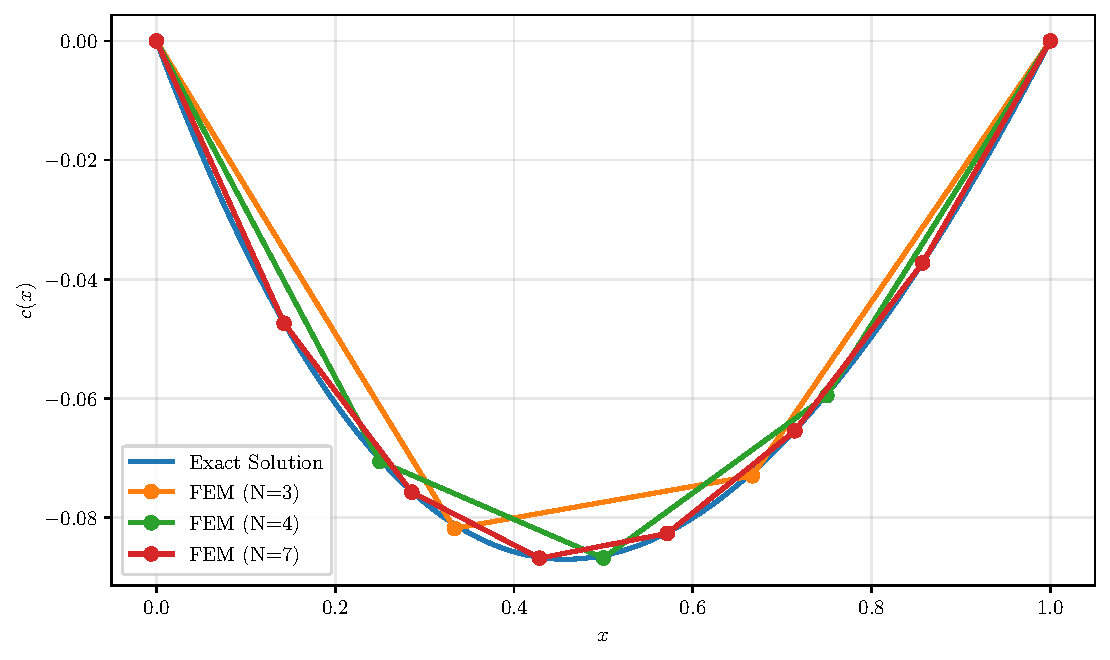
\includegraphics[width=0.6\textwidth]{figs/ode/fem_convergence.pdf}
    \caption{Finite element method solution to $c'' - c = \exp(-x^2)$. Using piecewise linear tent basis functions, the solution converges rapidly. Even with a small number of elements ($N=3, 4, 7$), the method captures the curvature of the solution effectively.}
    \label{fig:fem_convergence}
\end{figure}

The finite element method thus combines the best of both worlds: (1) the geometric flexibility and sparse matrix structure of finite differences, and (2) the error minimization and integral formulation of weighted residual methods.

\subsection{The Finite Volume Method}

FEM is very clean mathematically (same functions for both the expansion and the testing), but in a lot of transport problems, we really want to build conservation in by construction. That is the motivating idea behind the finite volume method: instead of asking for the residual to be orthogonal to the same tent functions, we ask for the residual to have zero \emph{average} over a little control volume around each node. You can still think of this as a Galerkin/weighted-residual method, but with a different set of test functions, the \textit{conjugate basis functions}. To be explicit, we keep the same piecewise-linear approximation for the solution using the tent functions $\{\Phi_i\}_{i=1}^{M-1}$,
\begin{equation}
    c(x) \approx \sum_{j=1}^{M-1} c_j \Phi_j(x)
\end{equation}
so $c(x)$ is continuous and varies linearly between nodes. The change is the test function. For each interior node $x_i=i\Delta x$, we associate a control volume that extends halfway to the neighboring nodes; it is convenient to denote its faces by
\begin{equation}
    x_{i-1/2} = x_i - \frac{\Delta x}{2},
    \qquad
    x_{i+1/2} = x_i + \frac{\Delta x}{2}
\end{equation}
The conjugate basis function $\Psi_i$ is just a normalized top-hat on that control volume (so integrals become averages):
\begin{equation}
    \Psi_i(x) =
    \begin{cases}
        \dfrac{1}{\Delta x}, & (i-\tfrac{1}{2})\Delta x < x < (i+\tfrac{1}{2})\Delta x,\\[10pt]
        0, & \text{otherwise}
    \end{cases}
\end{equation}

\begin{figure}[H]
    \centering
    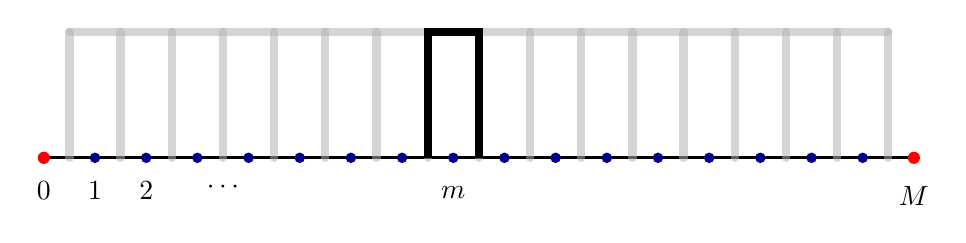
\begin{tikzpicture}[x=0.65cm,y=1cm]
        % parameters
        \def\M{17}    % right endpoint index (labeled M)
        \def\m{8}     % highlighted cell index (labeled m)
        \def\H{1.6}   % height

        \pgfmathtruncatemacro{\MMone}{\M-1}

        % baseline
        \draw[line width=1.2pt] (0,0) -- (\M,0);

        % background "box" grid: verticals at half-integers + top bar
        \draw[gray!60,opacity=0.55,line width=3.0pt,line cap=round]
        (0.5,\H) -- ({\M-0.5},\H);

        \foreach \k in {0,...,\MMone}{
        \draw[gray!60,opacity=0.55,line width=3.0pt,line cap=round]
            ({\k+0.5},0) -- ({\k+0.5},\H);
        }

        % highlighted box over cell m : [m-1/2, m+1/2]
        \draw[line width=2.8pt, line join=miter] ({\m-0.5},0) -- ({\m-0.5},\H) -- ({\m+0.5},\H) -- ({\m+0.5},0);

        % nodes on the line
        \fill[red] (0,0) circle (2.2pt);
        \fill[red] (\M,0) circle (2.2pt);
        \foreach \i in {1,...,\MMone}{
        \fill[blue!55!black] (\i,0) circle (1.9pt);
        }

        % labels
        \node[below=5pt] at (0,0) {$0$};
        \node[below=5pt] at (1,0) {$1$};
        \node[below=5pt] at (2,0) {$2$};
        \node[below=5pt] at (3.5,0) {$\cdots$};
        \node[below=7pt] at (\m,0) {$m$};
        \node[below=7pt] at (\M,0) {$M$};
    \end{tikzpicture}
    \caption{Finite volume method conjugate basis functions (control volumes).}
    \label{fig:fvm_conjugate_basis_functions}
\end{figure}

Now, we apply this to our model problem
\begin{equation}
    \frac{d^2 c}{dx^2} - c = \exp(-x^2), \qquad c(0)=c(1)=0
\end{equation}
The weighted residual statement with the conjugate test function is
\begin{equation}
    \int_0^1 \left[\frac{d^2 c}{dx^2} - c\right]\Psi_i(x)\,dx
    =
    \int_0^1 \exp(-x^2)\,\Psi_i(x)\,dx,
    \qquad i=1,2,\dots,M-1
\end{equation}
and because $\Psi_i$ is only nonzero on the control volume, this is just the local averaged balance
\begin{equation}
    \frac{1}{\Delta x}\int_{x_{i-1/2}}^{x_{i+1/2}}
    \left[\frac{d^2 c}{dx^2} - c\right]\,dx
    =
    \frac{1}{\Delta x}\int_{x_{i-1/2}}^{x_{i+1/2}} \exp(-x^2)\,dx
\end{equation}
The second derivative term turns into a clean flux difference automatically (this is the conservation-law flavor showing up). Using the fundamental theorem of calculus,
\begin{equation}
    \frac{1}{\Delta x}\int_{x_{i-1/2}}^{x_{i+1/2}} \frac{d^2 c}{dx^2}\,dx
    =
    \frac{1}{\Delta x}\left[\left.\frac{dc}{dx}\right|_{x_{i+1/2}} - \left.\frac{dc}{dx}\right|_{x_{i-1/2}}\right]
\end{equation}
Since our approximation is linear on each interval, $\frac{dc}{dx}$ is constant on each cell, so the face slopes are the usual two-point slopes:
\begin{equation}
    \left.\frac{dc}{dx}\right|_{x_{i+1/2}} \approx \frac{c_{i+1}-c_i}{\Delta x},
    \qquad
    \left.\frac{dc}{dx}\right|_{x_{i-1/2}} \approx \frac{c_i-c_{i-1}}{\Delta x}
\end{equation}
Plugging these into the flux difference gives the familiar central-difference stencil (but now it came from a flux balance, not Taylor series):
\begin{equation}
    \frac{1}{\Delta x}\left[\left.\frac{dc}{dx}\right|_{x_{i+1/2}} - \left.\frac{dc}{dx}\right|_{x_{i-1/2}}\right]
    \approx
    \frac{1}{(\Delta x)^2}\left(c_{i+1}-2c_i+c_{i-1}\right)
\end{equation}
The other term is the ``volume-averaged reaction'' piece. In the integrated equation, it appears as
\begin{equation}
    -\frac{1}{\Delta x}\int_{x_{i-1/2}}^{x_{i+1/2}} c(x)\,dx
\end{equation}
and we evaluate it by substituting the same tent-function expansion
\begin{equation}
    c(x) \approx \sum_{j=1}^{M-1} c_j\Phi_j(x)
\end{equation}
Over the control volume $[x_{i-1/2},x_{i+1/2}]$, only $\Phi_{i-1}$, $\Phi_i$, and $\Phi_{i+1}$ overlap, so the integral reduces to those three coefficients. Carrying out the little ``rectangle meets triangle'' area calculation gives
\begin{equation}
    -\frac{1}{\Delta x}\int_{x_{i-1/2}}^{x_{i+1/2}} c(x)\,dx
    \approx
    -\frac{1}{8}\left(c_{i+1}+6c_i+c_{i-1}\right)
\end{equation}
Intuitively, this is a weighted average over the volume: the center node gets weight $6/8$ and the neighbors get $1/8$ each, because the control volume cuts through the tent shapes at half-height. On the right-hand side, we just get the control-volume average of the source term:
\begin{equation}
    \frac{1}{\Delta x}\int_{x_{i-1/2}}^{x_{i+1/2}} \exp(-x^2)\,dx
\end{equation}
which you can evaluate numerically (Gaussian quadrature, etc.). Putting the flux term and the volume-averaged terms together, the FVM discretization for each interior node is
\begin{equation}
    \frac{1}{(\Delta x)^2}\left(c_{i+1}-2c_i+c_{i-1}\right)
    - \frac{1}{8}\left(c_{i+1}+6c_i+c_{i-1}\right)
    =
    \frac{1}{\Delta x}\int_{x_{i-1/2}}^{x_{i+1/2}} \exp(-x^2)\,dx,
    \qquad i=1,2,\dots,M-1
\end{equation}
The boundary conditions still just fix the endpoint coefficients,
\begin{equation}
    c_0=0,
    \qquad
    c_M=0
\end{equation}
so, just like FEM, we end up with a sparse tridiagonal linear system $\mathbf{A}\mathbf{c}=\mathbf{b}$ (only $c_{i-1}$, $c_i$, $c_{i+1}$ show up in the $i$th equation). The main difference is \emph{where the stencil comes from}: FVM is literally enforcing a control-volume balance (flux in/out + volume-averaged reaction = volume-averaged source), which is why it's so popular in transport and fluids.

\begin{figure}[H]
    \centering
    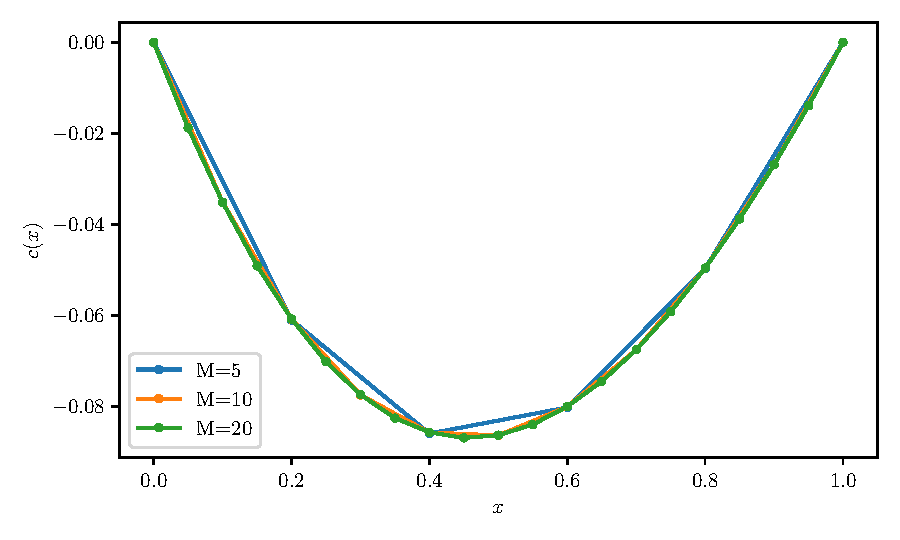
\includegraphics[width=0.6\textwidth]{figs/ode/fvm_convergence.pdf}
    \caption{Finite volume method solution ($M=5,10,20$) for the same problem as FEM. While the curve looks similar to FEM, the coefficients in the underlying matrix differ slightly due to the specific averaging properties of the rectangular test functions.}
    \label{fig:fvm_results}
\end{figure}

\section{Summary of BVP Methods}

We've looked at several families of BVP solvers, and a useful way to compare them is by the mental model each method imposes on the problem: do you treat the BVP like an IVP, do you approximate the operator directly, or do you enforce the equation in an averaged/projection sense?

The shooting method reframes a boundary value problem as a sequence of initial value problems. You guess the missing initial condition(s), integrate forward with an ODE solver, and then adjust the guess so that the terminal boundary condition is satisfied (often using a Newton or secant update built from the mismatch at the far boundary). When it works, it's conceptually straightforward and takes great advantage of the robustness of IVP integrators, but it can become delicate as the domain grows or the dynamics become stiff. In these cases, small errors in the ``aim'' can amplify exponentially, and multiple solutions (or unstable manifolds) can make convergence very sensitive to the initial guess.

The finite difference method stays closest to the differential equation itself. You put down a mesh, replace derivatives by difference quotients derived from local Taylor expansions, and solve the resulting algebraic system. This is typically the quickest path from PDE/ODE to code on a simple 1D domain, and it produces sparse banded matrices with predictable structure. The main limitations show up when the geometry, coefficients, or boundary conditions stop being simple: complex boundaries, strong coefficient variation, and nonuniform meshes require more bookkeeping, and it's easy to lose consistency or accuracy if stencils aren't adapted carefully.

In basis-function expansions (spectral methods), you take the opposite stance: instead of local stencils, you approximate the solution globally as a combination of smooth basis functions (Fourier modes, Chebyshev polynomials, eigenfunctions, etc.). For smooth solutions on simple domains, this can be extraordinarily accurate; errors often drop faster than any fixed algebraic order as you increase the number of modes. The tradeoff is that the discretization tends to couple many degrees of freedom at once, which leads to dense matrices (or global transforms) and makes complicated geometries, sharp layers, discontinuities, or highly localized features more challenging without additional machinery.

The finite element method builds the approximation from local pieces (low-order polynomials on elements) and enforces the equation in a weak (integral) sense by testing against the same basis functions (Galerkin). This perspective naturally handles variable coefficients, complicated geometries (in higher dimensions), and mixed boundary conditions. Yet, it still preserves a clear notion of stability and error control through functional analysis. In practice, FEM's strength is that it gives you a principled way to construct sparse systems with good approximation properties and a rigorous framework for refinement and convergence.

Finally, the finite volume method is closest to a conservation-law viewpoint. You still represent the solution with local degrees of freedom, but you enforce the governing equation by integrating it over control volumes. Equivalently, you test against piecewise-constant ``top-hat'' functions. This makes the discrete equations read like a physical balance: flux in minus flux out plus any volumetric production/consumption equals the volumetric source. That structure is exactly why FVM dominates in transport and fluid problems. In the FVM, conservation is built in by construction, and it remains meaningful even when coefficients are discontinuous or the solution develops sharp gradients.

\section{Exercises}

\begin{exercise} % 2020 Participation quiz L18
    Suppose we are solving a BVP using the Shooting Method. If an initial guess $c$ gives a result $x(\tau; c) > x_f$, where $x(\tau) = x_f$ is the boundary condition for
    \[
        \frac{dx}{dt} = g(f(t), t)\qquad t\in [0,\tau]
    \]
    and the sensitivity, $S(\tau; c)$, is negative, would the Shooting Method suggest to increase or decrease $c$?
\end{exercise}

\begin{solution}
    In first order approximation (Newton's method):
    \[
        \tilde{x}(\tau;c+\Delta c) = x(\tau; c) + \delta(c;\tau)\Delta c
    \]
    \(\Rightarrow\) Choose \(\Delta c\) st. \(\tilde{x}(\tau;c+\Delta c) = x_f \Rightarrow \Delta c = \dfrac{x_f-x(\tau;c)}{\delta(c;\tau)}\)\\
    Thus, the \fbox{shooting method suggests \underline{\underline{increasing}} \(c\)!}
\end{solution}

\begin{exercise} % 2020 Participation quiz L19
    If we are using collocation to approximate the solution of
    \[
        \frac{dx}{dt} = f(x(t),t) \qquad g(x(t_0), x(t_f)) = 0
    \]
    using
    \[
        x(t) = \sum_{i=1}^N c_i \cos \left(\frac{i\pi t}{t_f-t_0}\right),
    \]
    how many collocation points, \{\(t_i\)\}, do we need to choose?
\end{exercise}

\begin{solution}
    Let the state \(x\) be \(M\)-dimensional. (\(M\) could be 1, in the case of a scalar state.) Then, there are \underline{\underline{\(M\cdot N\) unknowns}} \(c_i \in\mathbb{R}^M,\, i=1,\cdots, N\) in the truncated series expansion. Without any further information, we shouldn't assert that any of the BCs is implied by the choice of basis functions.

    Thus, we need to pick \fbox{\(N-1\) collocation points} to obtain a square equation system:
    \[
        \begin{array}{llr}
        \dfrac{dx}{dt}(t_i) = f\left(x(t_i),t_i\right),\quad i = 1,\dots,N-1  & \qquad\longrightarrow\qquad & M(N-1) \text{ equations}\\[10pt]
        g\left(x(t_0),x(t_f)\right) = 0                                       & \qquad\longrightarrow\qquad & M \text{ equations}\\[4pt]
              \cline{3-3}\\[-8pt]
          & & M \cdot N \text{ equations}
        \end{array}
    \]
\end{solution}

\begin{exercise} % 2025 "Final extra problems" Nathan Morgan
    (*) Consider the following initial value problem:
    \[
        \frac{dx}{dt} = -x, \qquad x(0) = x_0.
    \]
    \begin{enumerate}[label=(\alph*)]

        \item Derive a linear system whose solution gives $x$ at each
        grid point.  Use a step size of $\Delta t$, a centered
        2nd-order finite difference for the interior points, and a
        backward 1st-order finite difference for the final point.

        \item What is the sparsity pattern of the resulting linear
        system?  Is there a relevant algorithm for solving systems
        with this structure?  How does the computational complexity
        scale with $\Delta t$ when the simulation horizon $[0, T]$ is
        fixed?

    \end{enumerate}
\end{exercise}

\begin{solution}
    \begin{enumerate}[label=(\alph*)]

        \item Using the centered second-order finite difference for the
        time derivative at interior nodes:
        \[
            \frac{x_{i+1}-x_{i-1}}{2\Delta t}
            \approx \left.\frac{dx}{dt}\right|_{x_i} = -x_i.
        \]
        Rearranging gives the discrete algebraic equation
        \[
            (-1)\,x_{i-1} + (2\Delta t)\,x_i + (1)\,x_{i+1} = 0.
        \]
        Our vector of unknowns is
        \[
            \mathbf{x} = \begin{pmatrix} x_1 \\ x_2 \\ \vdots \\ x_N
            \end{pmatrix}.
        \]
        From this we get, in the notation of
        Exercise~\ref{ex:thomas-algorithm}, $a_i = -1$, $b_i = 2\Delta t$,
        and $c_i = 1$, with $a_0 = 0$ because of the boundary conditions.

        % Note: the i=1 equation below is written with x_i rather than
        % x_1, and the first row of A drops the -1 that was moved to the RHS.
        For the case $i = 1$ our equation is
        \[
            \frac{x_{i+1} - x_0}{2\Delta t} \approx -x_i,
        \]
        which rearranges to
        \[
            (2\Delta t)\,x_i + (1)\,x_{i+1} = x_0.
        \]
        This gives $d_1 = x_0$.

        For the case $i = N$, we use
        \[
            \frac{x_N - x_{N-1}}{\Delta t} \approx -x_N,
        \]
        which rearranges to
        \[
            (-1)\,x_{N-1} + (1 + \Delta t)\,x_N = 0.
        \]

        Then the linear system $A\mathbf{x} = \mathbf{b}$ has
        \[
        A =
        \begin{pmatrix}
        2\Delta t & 1          &        &            &               \\
        -1        & 2\Delta t  & 1      &            &               \\
                  & \ddots     & \ddots & \ddots     &               \\
                  &            & -1     & 2\Delta t  & 1             \\
                  &            &        & -1         & (1+\Delta t)
        \end{pmatrix},
        \qquad
        \mathbf{b} =
        \begin{pmatrix}
            x_0 \\[4pt] 0 \\[4pt] \vdots \\[4pt] 0 \\[4pt] 0
        \end{pmatrix}.
        \]

        \item The system is tridiagonal: each equation couples $x_i$
        only to its neighbors $x_{i-1}$ and $x_{i+1}$.  The relevant
        algorithm is the Thomas algorithm from
        Exercise~\ref{ex:thomas-algorithm}, which solves a tridiagonal
        system in $\mathcal{O}(N)$ operations.  With the horizon
        $[0, T]$ fixed, the number of grid points is $N = T/\Delta t$,
        so the cost scales as $\mathcal{O}(1/\Delta t)$: halving the
        step size doubles the work.

    \end{enumerate}
\end{solution}

% Commented out per review.
% \begin{exercise} % 2025 Review 3 Nathan Morgan
%     Consider the boundary value problem
%     \[
%         \frac{d\mathbf{x}}{dt} = \mathbf{f}(\mathbf{x}, t), \quad \mathbf{g}(\mathbf{x}(t_0), \mathbf{x}(t_f)) = \mathbf{0}.
%     \]
%     Since $\mathbf{x}(t_f)$ is determined by $\mathbf{x}(t_0)$ through the ODE, $\mathbf{g}$ can be viewed as a function of $\mathbf{x}(t_0)$ alone. Write $\mathbf{g}(\mathbf{x}(t_0))$ explicitly when the boundary conditions are $x_1(t_0) = 1$ and $x_2(t_f) = 3$. You can use $\mathrm{ode}(\mathbf{f}, \mathbf{x}(t_0), [t_0, t_f])$ to denote the solution of the ODE integrated from $t_0$ to $t_f$ with initial condition $\mathbf{x}(t_0)$
% \end{exercise}
%
% \begin{solution}
%     \[
%         \mathbf{g}(\mathbf{x}(t_0)) =
%         \begin{bmatrix}
%             (\mathbf{x}(t_0))_1 - 1 \\[4pt]
%             \mathrm{ode}(\mathbf{f},\,\mathbf{x}(t_0),\,[t_0,\,t_f]) - 3
%         \end{bmatrix}
%     \]
% \end{solution}

\begin{exercise} % 2025 Review 3 Nathan Morgan
    Classify each of the following as Dirichlet, Neumann, Robin, or none of these.
    \begin{enumerate}[label=(\alph*)]
        \item $\displaystyle x(0)\cdot\left.\frac{dx}{dt}\right|_{t=0} = 1$.
        \item For the ODE $\dfrac{d^2C}{dx^2} = -r(C)$, the condition $C'(0) = 1$.
    \end{enumerate}
\end{exercise}

\begin{solution}
    \begin{enumerate}[label=(\alph*)]
        \item None of the three types. The condition is nonlinear since it involves the product of the solution and its derivative.
        \item Neumann: the value of the first derivative $C'$ is specified at the boundary $x = 0$.
    \end{enumerate}
\end{solution}

% Commented out per review.
% \begin{exercise} % 2025 Review 3 Nathan Morgan
%     Implement the shooting method in MATLAB for the general boundary value problem
%     \[
%         \frac{d\mathbf{x}}{dt} = \mathbf{f}(\mathbf{x}, t), \quad \mathbf{g}(\mathbf{x}(t_0), \mathbf{x}(t_f)) = \mathbf{0}.
%     \]
%     Assume \texttt{f} and \texttt{g} are defined as MATLAB functions and that \texttt{t0}, \texttt{tf}, and an initial guess \texttt{c0} for the initial condition $\mathbf{x}(t_0)$ are available in the workspace.
% \end{exercise}
%
% \begin{solution}
%     \lstinputlisting{code/matlab/ode/shoot.m}
% \end{solution}

\begin{exercise} % 2025 Review 3 Nathan Morgan
    Let $\mathbf{S} = \dfrac{\partial\mathbf{x}(T)}{\partial\mathbf{c}}$ be the sensitivity matrix of the ODE solution at the final time with respect to the initial condition $\mathbf{c} = \mathbf{x}(t_0)$, for the BVP $\dfrac{d\mathbf{x}}{dt} = \mathbf{f}(\mathbf{x},t)$, $\mathbf{g}(\mathbf{x}(t_0), \mathbf{x}(T)) = \mathbf{0}$.
    \begin{enumerate}[label=(\alph*)]
        \item Why is $\mathbf{S}$ useful when applying the shooting method?
        \item Describe two methods for computing $\mathbf{S}$.
        % \item For a scalar problem, $c = 1$ gives $x(T) = 1.0$ and $c = 1.0001$ gives $x(T) = 1.123$. Compute $\partial x/\partial c$ numerically.
    \end{enumerate}
\end{exercise}

\begin{solution}
    \begin{enumerate}[label=(\alph*)]
        \item $\mathbf{S}$ is useful for two reasons. First, it enables computation of the Jacobian of the shooting residual $\mathbf{g}$ with respect to $\mathbf{c}$:
        \[
            \mathbf{J} = \nabla_{\mathbf{c}}\bigl(\mathbf{g}(\mathbf{x}(t_0)=\mathbf{c},\,\mathbf{x}(T)(\mathbf{c}))\bigr) = \frac{\partial\mathbf{g}}{\partial\mathbf{c}} + \frac{\partial\mathbf{g}}{\partial\mathbf{x}}\,\mathbf{S}.
        \]
        This tells us (to first order) how to update $\mathbf{c}$ to reduce the residual and whether the solution $\mathbf{c}^*$ is locally unique. Second, examining $\mathbf{J}$ at a candidate $\mathbf{c}^*$ can explain why \texttt{fsolve} failed to converge.
        \item Two methods for computing $\mathbf{S}$:
        \begin{enumerate}[label=\roman*.]
            \item \textit{Numerical differentiation}: perturb each component of $\mathbf{c}$, solve the ODE for each perturbation, and estimate each column of $\mathbf{S}$ by finite differences.
            \item \textit{Sensitivity ODE}: differentiate the ODE with respect to $\mathbf{c}$ to obtain a matrix-valued ODE-IVP for $\mathbf{S}$, solved alongside the original ODE.
        \end{enumerate}
        % \item Using a forward finite difference:
        % \[
        % \frac{\partial x}{\partial c} \approx \frac{x(T)\big|_{c=1.0001} - x(T)\big|_{c=1}}{1.0001 - 1} = \frac{1.123 - 1.0}{0.0001} = 1{,}230.
        % \]
    \end{enumerate}
\end{solution}